%! TEX root = ../../main.tex

\subsection{Microservices}%
\label{sub:Microservices}

There exist many different definitions of the term \textit{microservice}.
\autocite{DragoniMicroservicesyesterdaytoday2016} defines a microservice to be
a \enquote{cohesive, independent process interacting via messages}. The
definition of \autocite{MikeAmundsenMicroserviceArchitecture2016} also takes
the architectural aspect into account stating that a \textit{microservice
architecture} is \enquote{style of engineering highly automated, evolvable
software systems made up of capability-aligned microservices}. Regardless of
the specific definition, one common concept becomes clear: A microservice
should be a small independent piece of software that communicates using
messages and can be deployed autonomously.

This chapter will cover the origins of the microservice architecture, introduce
a practical example of a microservice and outline the problems that need to be
addressed when deploying a microservice.

\subsubsection{History}%
\label{ssub:History}

When designing an application, one option is to use a monolithic architecture.
A monolithic application is developed by one big group of developers and the
source code is maintained inside a single repository. The monolithic
application offers a number of functionalities (also called \textit{services})
that can be consumed. A team of operators is responsible to deploy and manage
the application so that it can be consumed \autocite[p.
584]{VillamizarEvaluatingmonolithicmicroservice2015}. The services of a
monolith can not be executed independently from one another. Hence, a monolith
exists as a single executable artefact \autocite[p.
1]{DragoniMicroservicesyesterdaytoday2016}.

Monolithic applications are hard to deploy in a distributed system without
introducing some kind of middleware that handles the way the monolith is
distributed. In addition to this, monolithic application suffer additional
drawbacks. Maintaining a monolith can pose a big problem due to its huge code
base and many internal and external dependencies. Furthermore, deploying a new
version can cause major downtimes since the whole application has to be
(re)started. From a development standpoint, monoliths also pose the problem of
restricting the technology stack once it has been defined. This can produce an
environment that is now longer suitable for all new services added to the
monolith. Lastly scaling a monolith is not possible indefinitely \autocite[p.
2]{DragoniMicroservicesyesterdaytoday2016}. When scaling an application
\textit{vertically}, resources (e.g.\ RAM) are added to the machine executing
the application. Contrary to this approach, when scaling \textit{horizontally}
the application gets distributed onto a number of machines. This however
requires the use of a distributed middleware or code changes \autocite[Ch.
1.1.1]{LuksaKubernetesAction2017}.

The \ac{SOA} solves a lot of the problems afflicting the monolithic
architecture. Rather than providing all services as part of one application, in
\ac{SOA} the application is split up into multiple small \textit{business
applications} that each offer only a small hand of services. Each business
application is maintained by a specialised development team. The business
applications offer their services to other services or directly to consumers
through a set of protocols; the primarily used protocol is \ac{SOAP}. The
operation of all business applications is handled by a separate operations
teams \autocite[p.  584]{VillamizarEvaluatingmonolithicmicroservice2015}.

Even though the \ac{SOA} approach does solve a lot of problems the monolithic
architecture suffers from, several problems remain. Implementing the \ac{SOA}
into existing and new applications can be difficult resulting in hight costs.
Additionally the technology that is needed to route the requests to the correct
business application is not designed to run inside a modern cloud environment
\autocite[p. 584]{VillamizarEvaluatingmonolithicmicroservice2015}.

The goal of the microservice architecture is to adopt the advantages of the
\ac{SOA} while solving the problems the monolith architecture suffers from
\autocite[p. 584]{VillamizarEvaluatingmonolithicmicroservice2015}.

\autocite{VillamizarEvaluatingmonolithicmicroservice2015} proposes the
questions whether the microservice architecture is a new architectural style or
simply another term for the already existing \ac{SOA}.
\autocite{VillamizarEvaluatingmonolithicmicroservice2015} concludes that the
microservice architecture can be viewed as a subset of the \ac{SOA}. Besides
that it additionally focuses on greater agility. Altogether,
\autocite{DragoniMicroservicesyesterdaytoday2016} defines the microservice
architecture to be a distributed application which \textit{modules} are only
microservices. The term \enquote{module} is synonymous with the term
\enquote{service} used in the description of the monolithic architecture and
\ac{SOA}.

Furthermore, the user does not contact any service directly. One or more
gateways receives the user's requests and route them to the correct service.
Depending on the type of user, the requested information are encoded
appropriately by the gateway. An end user might receive a rendered website over
\ac{HTTP} whereas an \ac{API} call has to be sent via \ac{REST} over \ac{HTTP}.
The operation of said gateway is managed by an independent team \autocite[p.
585]{VillamizarEvaluatingmonolithicmicroservice2015}. Two common approaches in
this field are \ac{API} gateways and service meshes. Their properties and
respective advantages are further discussed in
\autocite{HariharaSubramanianHandsRESTfulAPI2019}.

In summary it can be said that the microservice architecture constitutes the
natural evolution of software architectural patterns in a distributed system.

\subsubsection{A Practical Example}%
\label{ssub:A_Practical_Example}

The following example highlights the advantages of microservice in a practical
environment. The example depicts an application that allows users to share
pictures of their pets with other users; hereafter called \textit{PawPic}.
It is a requirement that all users have to be authenticated using an external
\textit{Active Directory} system in order to to view and post pictures.

Following the concept of \textit{cohesion} \autocite[p.
2]{DragoniMicroservicesyesterdaytoday2016}, any service only provides the
functionality that is needed to solve the specific problem it is assigned to
solve. Figure~\ref{fig:microservice_example} proposes a microservice
architecture for the \textit{PawPic} application.

\begin{figure}[H]
\begin{center}
  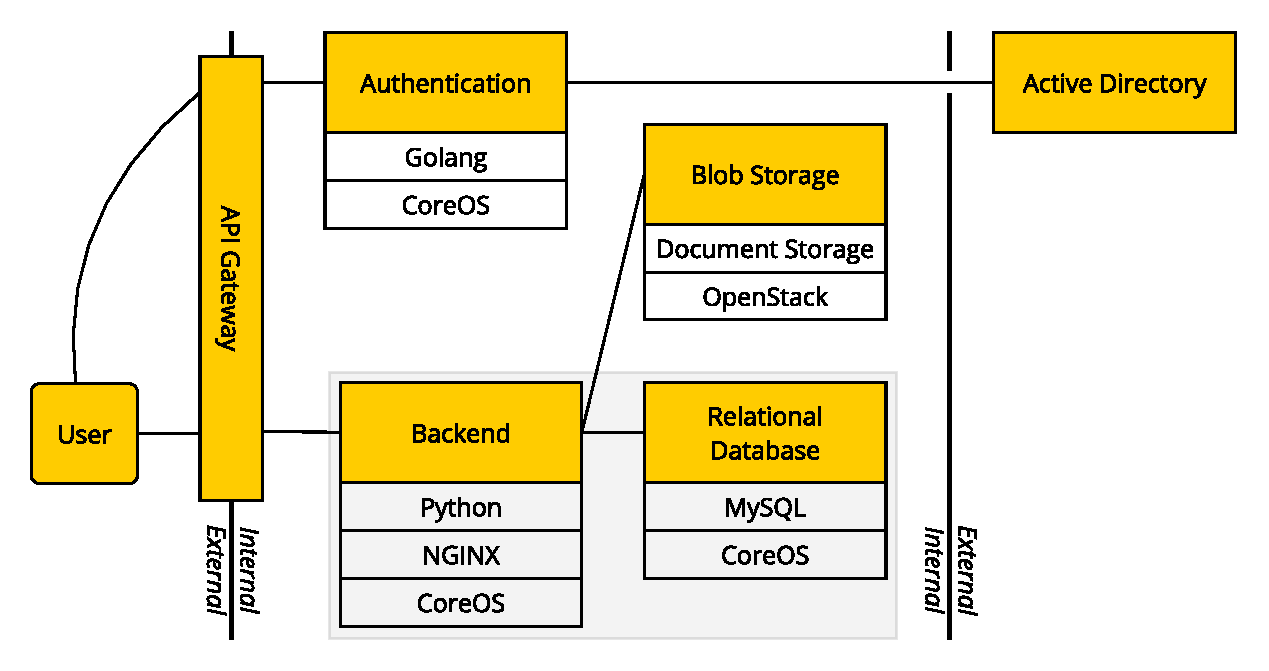
\includegraphics[scale=0.7]{images/figures/microservice_example.pdf}
\end{center}
\caption{A basic microservice architecture example containing three internal
service, one external service and an \acs{API} gateway.}
\label{fig:microservice_example}
\end{figure}

The proposed architecture includes an \ac{API} gateway that handles all requests
targeted at one of the internal services. This only applies to requests by a
user and does not include requests an internal service performs towards an
external service.

The architecture further contains three internal services only two of which can
be directly targeted by the user; the authentication and backend service. The
authentication service's only purpose is to check the user's credentials.
Besides that, the backend service provides the applications main functionality;
to view and share pictures of pets. To fulfil this task, the backend uses a
relational database. The database holds the picture's information and storage
metadata. Both the backend and database are separate service though they are
strongly dependent on one another. Using the storage metadata, the backend is
able to fetch the actual images from the blob storage service and relay them to
the user.

With the introduction of new features it must be decided whether the new
features still solve the problem of viewing and posting pictures of pets. If
this is not the case, a new service must be introduced. This ensures that each
service still follows the concept of cohesion.

The service's technology stacks are fully independent from one another. The
authentication service e.g.\ is written in Golang due to the high performance
the language offers. The backend however is written in Python and runs on top
of a NGINX server. This approach does not lock the developers in one technology
stack that might not suite the problem's needs in the future. In addition,
every service can be scaled independently from one another. 

\subsubsection{Deployment -- A Software-based View}%
\label{ssub:Deployment_-_A_Software-based_View}

\subsubsection{Problems}%
\label{ssub:Problems}


